% *** Authors should verify (and, if needed, correct) their LaTeX system  ***
% *** with the testflow diagnostic prior to trusting their LaTeX platform ***
% *** with production work. IEEE's font choices can trigger bugs that do  ***
% *** not appear when using other class files.                            ***
% The testflow support page is at:
% http://www.michaelshell.org/tex/testflow/

\newcommand{\todo}[1]{\textbf{TODO: #1}}

\documentclass[conference]{IEEEtran}

\usepackage{url}
\usepackage{graphicx}
% correct bad hyphenation here
\hyphenation{op-tical net-works semi-conduc-tor}

\begin{document}
\title{Spreadsheets are Code}

\author{\IEEEauthorblockN{Felienne Hermans, Bas Jansen, Sohon Roy, Efthimia Aivaloglou, David Hoepelman and Alaaeddin Swidan}
\IEEEauthorblockA{f.f.j.hermans, \todo{emailadresses}}
\IEEEauthorblockA{Delft University of Technology, the Netherlands}
}


\maketitle

\begin{abstract}
The abstract goes here.
\end{abstract}

\IEEEpeerreviewmaketitle

\section{Introduction}
Spreadsheets are used for a large variety of different tasks, from invoicing to planning and from budgeting to scheduling, in all sorts of domains, from small shops to multinationals. In 2004, the International Data Corporation interview 118 business leaders and found that 85\% were using spreadsheets in financial reporting and forecasting~\cite{Panko2008} Especially in the financial domain, spreadsheets are ubiquitous. Financial intelligence firm CODA reported in 2008 that 95\% of all U.S. companies use spreadsheets for financial reporting~\cite{Panko2008}. The number of end-user programmers in the USA alone is conservatively estimated at 11 million, compared to only 2.75 million other, professional programmers~\cite{Scaf2005}. 

In a survey~\cite{BLS2003} held in 2003 by the US Bureau of Labor Statistics, over 60\% of 77 million surveyed workers in the US reported using spreadsheets, making this the third most common use of computers, after email and word processing. A more recent survey among 95 companies world-wide placed spreadsheets on the fourth place after email, browsing and word processing, accounting for 7.4\% of computer time~\cite{Wellnomics2007}. The Dutch Bureau of Statistics investigates computer literacy among Dutch civilians every year, and has reported a rise in people able to use formulas in a spreadsheet from 44\% to 54\% between 2006 and 2013~\cite{CBS2013}.




As artifacts of end-user programming, spreadsheets often play a role similar to source code in many companies: they support important organizational processes and sometimes even business decisions are taken based on the information they contain~\cite{Hermans2011}.

While spreadsheets are commonly used, their users often have little training as programmers, but in spite of that, they often face many of the challenges of professional developers, choosing which APIs, libraries, and functions to use~\cite{Ko2004}, or understanding someone else's code~\cite{Ko2011}. Since spreadsheets frequently contain errors~\cite{Panko1998}, end-users test, verify and debug their programs~\cite{Hermans2013-Cascon,Ko2004-Why}.

The above issues occurring in spreadsheets: program construction, maintenance, testing, debugging clearly occur in regular code bases too, and as such have been topics of research in the programming and software engineering community for decades~\cite{Ko2011}. Given these similarities between spreadsheets and source code, both in terms of application and issues, it is feasible to transform methods, tools and techniques from software engineering to spreadsheets, albeit sometimes in a form more tailored towards end-users. This exactly has been the approach of a number of researchers over the last decade, and this paper highlights their past achievements, challenges and future research directions. 


\section{End-user programming}
End-user programming has been a topic of study for decades, mainly started by by Nardi~\cite{Nardi1993} in her investigations into spreadsheet use in office workplaces. The difference between an end-user programmer and a professional programmer lies in their goals. It is the responsibility of a professional developer to build, debug, maintain and sometimes test software for others to use, while end-user developers create programs to support their own domain of expertise, like teaching, planning or bookkeeping~\cite{Ko2011}. As such, programs that end-users create are, by definition, not meant for others to use, while professional programming has the goal of producing code for others to use. 

The problematic aspects of end-user programming is that sometimes the created artifacts change from being a personal solution to a program used by many colleagues. When that happens, an end-user suddenly, often unintended and unprepared, has to take on challenges of professional developers, like testing, maintaining and generalizing their creations.

\section{Spreadsheets are Code}
While end-user programming can take on many forms, and their users can be as diverse as system administrators~\cite{Barrett2004}, interaction designers~\cite{Ko2004, brandt_opportunistic_2008, myers_how_2008}, spreadsheets can be considered the most successful form of end-user programming. 
 % Ko also names: natural scientists [Carver et al. 2007; Segal 2007], software architects [Lakshminarayanan et al. 2006], bioinformatics professionals [Letondal 2006], web designers [Rode and Rosson 2003]


As outlined above, spreadsheets are crucial tools for many workers, enabling millions of users to do reporting, planning, scheduling and all else needed to succeed in their jobs. Obviously, not all spreadsheets are full-fledged applications: some are simply used for word processing with an easier layout and do not even contain formulas. However, spreadsheet are also commonly used to create applications, or to perform business critical calculations. We argue this second group of spreadsheets can and should be seen as source code, paving the way to apply methods from software engineering to them. In the following, we will outline three reasons that spreadsheets systems are programming languages, and spreadsheet are code.

\subsection{Application domains are similar}
Firstly, spreadsheets are used for very similar problems, like financial calculations or data manipulation. In many cases, users have investigated the use of ‘off the shelf’ solution, however, they are often expensive and do not fit their needs exactly. A second alternative, having software made specifically for their problem tends to go over time and over budget as well. In that light, using a spreadsheets seems a cheap and simple solution for many end-users.

\subsection{Expressive power is similar}

\begin{figure}
  \begin{center}
  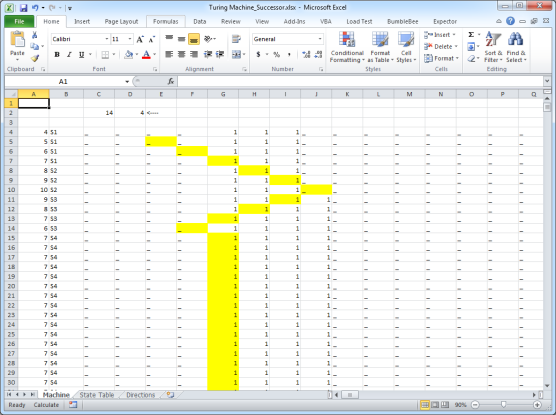
\includegraphics[width=\columnwidth]{fig/turing.png}
  \caption{A Turing machine implementation in Excel, using only formulas}
  \label{fig:visical}
  \end{center}
\end{figure} 

Secondly, spreadsheets are Turing complete, even when not take the Visual Basic for Applications code into account. Using formulas only, you can construct a Turing machine, see Figure \ref{fig:visical}~\cite{Turing2013}. 

\subsection{Maintainability issues are similar}

Finally spreadsheets suffer from typical software problems, including, but not limited to the issues below.

\textbf{Long life span} Sometimes, spreadsheets are created for one time use, and they are also thrown away after that use. More often they stay ‘alive’: enhanced with more data, reused for next year's budget or modified for a different department. Our research shows that spreadsheets have an average lifespan of five years~\cite{Hermans2011}.

\textbf{Many different users} During their lifespan, spreadsheets are frequently shared among coworkers. On average, twelve different people work with one spreadsheet during its life, in many different ways~\cite{Hermans2011}. Shared for data entry, for checking or for analysis.

\textbf{Lack of documentation} We found that only one in three spreadsheets  contain documentation, and we are not even talking about technical documentation, but just something as basic as a manual on how to use the spreadsheet is lacking in two thirds of the spreadsheets we examined.

\textbf{Quality issues} Many accounts of big impact errors: From somewhat silly errors, like an overbooked Olympic stadium\todo{link OS} to career wrecking data analysis mistakes\todo{link Reinhard}, the stories of errors are numerous. The European Risk Interest Group keeps a list of these ‘spreadsheet horror stories’ on their website\footnote{\url{www.eusprig.org/horror-stories}}

\section{Reflections on Spreadsheet Success factors}
Given the extreme wide adoption of spreadsheets, one could wonder why spreadsheets are as successful as they are. We believe there are a number of different reasons for their success.

\subsection{Live programming avant la lettre}

\begin{figure}
  \begin{center}
  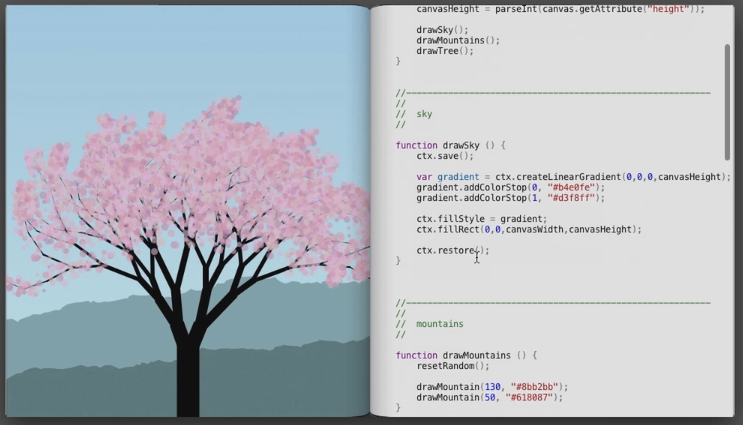
\includegraphics[width=\columnwidth]{fig/bret.png}
  \caption{Live programming: on the right the source code and on the left its instantiation of the code which changes immediately when the code is updated.}
  \label{fig:bret}
  \end{center}
\end{figure} 


Recently, ‘live programming’ has been made popular, among others by Bret Victor. Figure \ref{fig:bret} illustrates the idea of live programming. On the right, we have source code and on the right, we have the result of that code, in this case: a tree. Modifying the code will immediately affect the tree.
 
But this is exactly what happens in a spreadsheet. The minute we hit enter in a formula, we get the result. No compilation is needed. This liveness enables the flexibility that is often praised as the success factor of spreadsheets.

\subsection{Data, metadata and calculations in one view}
While researching spreadsheets, we have often asked the more tech savvy spreadsheet users why they did not use a more structured approach, like Microsoft Access. What we found was that the disconnect between the meta-data (designing the tables), the data (filling them) and the analysis (queries) was too hard for many users. The fact that all of those can be bundled in one view apparently makes it easier for non-programmers to keep an overview of what is going on. This is not that surprising, understanding dependencies of code is one of the challenges that developers still face, even advanced IDE's like Eclipse or Visual Studio do not solve this entirely. \todo{do we have a citation here?}

\subsection{One-click deployment}
Another problem that professional users face is the problem of deployment. Some more advanced users write, for example, Python scripts to analyze data. But how to get that to run on your neighbor's workstation, with a slightly different version of the operating system, a newer Office and different language settings? Spreadsheets are so universal that almost everyone has a spreadsheet program on their machine and the different programs can easily convert them. With that, a spreadsheet becomes an executable package with data and calculations packed together, that can run anywhere.

\section{Achievements} 
One of the approaches to \emph{end-user software engineering} research has been to transfer methods from software engineering to end-user languages, and this is an approach that has been applied eagerly in research into spreadsheets.  This section presents an overview of successful approaches following this scheme.

\subsection{Testing}
One of the programming concepts that found its way to spreadsheets earliest is testing. 

\todo{summarize WYSIWYT}



A third category of related work concerns the testing of spreadsheets. Centerpiece in this category is the work of Rothermel \emph{et al.}, who have created~\cite{Rothermel1997} and subsequently validated~\cite{Rothermel2000} a method to support end-users in defining and analyzing tests for spreadsheets. Their evaluation showed that their approach had an average fault detection percentage of 81\% which is ``comparable  to  those  achieved  by  analogous  techniques  for testing  imperative  programs." Other studies have confirmed the applicability of testing~\cite{Kruck2006}. The WYSIWYT methodology requires users to explicitly indicate what cells of a spreadsheet are correct and the system propagates the testedness of a cell to its dependents. Related is the elegant work of Burnett on spreadsheet assertions that uses a similar propagation system \cite{Burnett2003}.

\subsection{Documentation extraction} 
Like software, spreadsheets often suffer from a lack of documentation. In a field study, we found that only one in three spreadsheets have documentation~\cite{Hermans2011}. This seems to be a problem especially in situation where a spreadsheet was transferred: between colleagues, from a spreadsheet user to IT for migration or when a spreadsheet had to be reviewed by an auditor. To address the lack of documentation, we developed approaches to reverse engineers spreadsheets.

\subsubsection{Extracting class diagrams}
In this approach we attempted automatic extraction of class diagrams from spreadsheets. Spreadsheets contain groups of data, computations over these groups, and dependencies between them. This type of organization closely resembles that of object oriented systems, and thus groups of data were converted into classes, formulas into methods, and dependencies into associations. To achieve this conversion, we created a library of commonly used and well-defined spreadsheet patterns. We implemented the approach in a tool named \textit{Gyro}. The implementation was evaluated on the EUSES corpus. The patterns of the created library were found to be occurring in around 40\% of the corpus spreadsheets. For 50 randomly selected spreadsheets from the corpus, class diagrams were generated manually and compared with the output of the Gyro tool. In this also, 40\% of cases proved to be exact match and the rest had various degrees of mismatch with only 12\% being totally useless.

\subsubsection{Dataflow visualization}
We did a study in a large Dutch financial services company \textit{Robeco} to ascertain the types of information needs of industrial spreadsheet users. The results indicate that most important information needs of spreadsheet users concern the structure of formula dependencies. To meet this demand we conceived an approach for automatic generation of levelled data-flow diagrams from spreadsheets. The diagrams can be used to visualize data, processes that manipulate data, and the dependencies between them. Furthermore the diagrams can depict hierarchical structures like blocks of cells or different worksheets. We implemented the approach in a tool named \textit{GyroSAT}. It was evaluated with a group of 27 users from Robeco in the context of three transfer scenarios where spreadsheets were being transferred between users, from users to auditors, and from users to IT engineers who were migrating spreadsheets to custom software applications. The results indicate that the professionals from Robeco consider the tool helpful; the visualizations help them to create story lines for explaining spreadsheets to colleagues, and the visualizations scale well to large and complex spreadsheets in use at Robeco.

\subsection{Smell Detection} 
After focusing on extraction of documentation, we found out that spreadsheet users often prefer to work in spreadsheets over migrating them, hence we shifted our focus to helping users understand the complexity of spreadsheets and determine ways to improve them. For this, we took the idea of \emph{code smells} as inspiration, adapting it however, to be applicable to spreadsheets.

\subsubsection{Formula-level Smell detection}
We started by defining smells on the formula level where we found that many smell defined for code also applied nicely to spreadsheets. For example, conditional complexity can be applied as is, since spreadsheets support conditionals too. Some other smells needed some modification: many parameters became many references and long method became many operations. After defining the 

\subsubsection{Structural Smell detection}

\subsection{Clone detection}

\subsection{Improving/re-engineering/Refactoring}


\subsection{Conclusion}
This all has to do with understanding and improving quality we still want to support understanding domain/calculation.Our work and that of others was all 100\% automated, what we have learned, if we want to continue with reverse engineering, we need more support from the user, both the creator and human level intelligence (a generic user): we both want to do large studies with generic users like the labeling game and make support for users to add more (domain) knowledge to the sheets.

\section{Challenges} 

\subsection{End-users self perception}
One of the core challenges of researching spreadsheets, and also end-user programming in general is that users do not seen themselves as programmers. Therefore, they often do not have training, but this is not the core issue. We could provide them with training, but preferably we support them with easier and less error-prone methods with more expressive power to do their jobs.
The perception of end-user programmers as not being programmers is not limited to how programmers view themselves, but also to how they are seen by others. Professional developers and other coworkers of them often fail to recognize and often belittle their programming efforts.

\subsection{Lack of best practices}
A challenge that follows the previous one is the lack of standards. This inhibits easy processing of spreadsheets as it results in many differnt types of spreadsheets.

\subsection{Lack of data}
Spreadsheets often contain models and calculations of vital information to companies. As such, companies are often reluctant to share them with researchers. \todo{this is a broader issue in very applied/industrial research, tradeoff realism vs. reproducability} Even when we get large sets (like Enron), we do not have the users with them. There is no process data (version control history, like “MSR type papers”).

\subsection{Size of spreadsheets }
Spreadsheets can get big, navigating on 1 worksheet is still ok, but for larger sheets it is hard to filter what to present, just showing all dependencies is too much. [example from Enron, Sohon might have a pic]

For useful visualizatin, we have to leave the cell level, want to look at the computation level (slicing)

\todo{not sure what was meant here:}Getting domain knowledge out at a higher level, maybe with some assistance from the user, letting them know which cells have labels and which lack them.

\subsection{Performance}
Connection with size, \todo{Alaaeddin}

\subsection{Technical issues}
Finally, there are technical issues in processing spreadsheets and developing add-ins for a proprietary product like Microsoft Excel. 
Lack of open standards, and even when open, not very standardized (we have to reverse engineer stuff, link SCAM, also HPC/HEAT is not open, not willing to share)
Limited options for customization (undo/redo stack is not available, in the object model precedents do not go deeper than 1 level, objects model gets extended but not updated)

Obviously, one could steer away from these issues by implementing a system themselves (Forms/3 and Sestoft) or to build plugins for open source tools. Here however the tradeoff with realism is apparent too, building tools for Excel which is the number 1 spreadsheet solution increase the realism and impact of research tools.

\section{Future opportunities}
Given the above achievements  and challenges, we identify the following viable directions for future work.

\subsection{Continuation of the refactoring and testing work}
In contrast to the work on smells that have been tried in practice and spurred numerous follow up works and has been picked up by a larger research community, refactorings and testing need to be made more applicable.

\subsection{More deeply understanding the role of spreadsheets in the enterprise}
This understanding will have to happen both culturally (evolution, process) and in their application (use of spreadsheets) For example, classification different types of spreadsheets, potentially. For this we are exploring the following concrete endeavours:

\subsubsection{For the purpose of reverse engineering (Sohon)}
Potential application of extraction high level structure would be:
\paragraph{documentation extraction}
\paragraph{validating spreadsheets at a higher level}

\subsubsection{To support users in creating better spreadsheets}
Using  an alternative interface for some types of spreadsheets, bringing a higher level of abstraction (Bas)

\subsection{Beyond formulas}

  Self-service BI. This field is now mainly concerned with building but not with maintenance. We see them making the same mistake by not focusing on end-user maintenance, maybe underestimating the longevity of the new artifacts created. We suspect that this new incarnation of end-user programming again will suffer from smells etc. So our research will explore this, for example by focusing. Other spreadsheet concepts like PivotTables and VBA code
  

Increasing performance of spreadsheets (Allaeddin)
Intertwining of formulas and other constructs makes automated analysis even harder



\section{Conclusion}







% trigger a \newpage just before the given reference
% number - used to balance the columns on the last page
% adjust value as needed - may need to be readjusted if
% the document is modified later
%\IEEEtriggeratref{8}
% The "triggered" command can be changed if desired:
%\IEEEtriggercmd{\enlargethispage{-5in}}


\bibliographystyle{IEEEtran}
% argument is your BibTeX string definitions and bibliography database(s)
\bibliography{references}


% that's all folks
\end{document}


